\section{The Second Law of Thermodynamics}\label{sec:2nd_Law_Thermo}
\begin{definition}[\nth{2} Law of Thermodynamics]\label{def:2nd_Law_Thermo}
  The \emph{\nth{2} law of thermodynamics} states that the total \nameref{def:Entropy} of an \nameref{def:Isolated_System} can \textbf{never} decrease over time, and is constant if and only if all \nameref{def:Process}es are reversible.
  Isolated systems spontaneously evolve towards thermodynamic equilibrium, the state with maximum entropy.

  In terms of total \nameref{def:Energy} in a system, this law states that the total energy of the system is minimized at all times during a \nameref{def:Process}.

  \begin{remark}
    We do not discuss \nameref{def:Entropy} in this section.
    Rather, we discuss it in great detail in \Cref{sec:Entropy}.
  \end{remark}
\end{definition}

In more common terms, the \nameref{def:2nd_Law_Thermo} explains why some \nameref{def:Process}es only move in one direction.
For example, water going over a waterfall is \textit{technically} symmetric.
Meaning, that there is a chance the water will actually go back \textbf{up} the cliff.
However, the \nameref{def:2nd_Law_Thermo} explains that this reversal is so thermodynamically unfavorable that it will never happen.

Another example is a container of water that is greater than that of its surroundings.
For instance, the water is $\Temp = \SI{90}{\degreeF}$ and the surroundings are at $\Temp = \SI{20}{\degreeF}$.
The \nameref{def:2nd_Law_Thermo} explains why the heat always flows \textbf{out} of the water and to the surroundings, rather than the other way around.

This means that \textbf{energy is dispersed}.
This spread (dispersion) of energy is \nameref{def:Entropy}.

\begin{blackbox}
  \nameref{def:Energy} naturally flows from being concentrated in one place to another such that the dispersal of energy is maximized.
  This limits the \nameref{def:Work} that can be performed.
\end{blackbox}

\begin{definition}[Kelvin-Planck \nth{2} Law of Thermodynamics]\label{def:Kelvin_Planck-2nd_Law_Thermo}
  There are a variety of definitions of the \nth{2} law of thermodynamics.
  The one in \Cref{def:2nd_Law_Thermo} is just one of them.
  The \emph{Kelvin-Planck \nth{2} law of thermodynamics} states that it is impossible for any device that operates on a \nameref{def:Cycle} to receive heat form a single reservoir and use to to produce \nameref{def:Work}.

  \begin{remark}[Thermal Reservoir]\label{rmk:Thermal_Reservoir}
    A thermal source with a constant temperature.
    For example, the Earth, a large boiler, the air, a lake, or river are considered thermal reservoirs.
    More concretely, this means that if \nameref{def:Heat} is removed, there is no temperature change.
  \end{remark}
\end{definition}

\begin{definition}[Cycle]\label{def:Cycle}
  A \emph{cycle} is a \nameref{def:Process} whose ending state is the same as its starting state, allowing the process to continue again.

  \begin{remark}[Cyclic]\label{rmk:Cyclic}
    A \emph{cyclic} \nameref{def:Process} is one that behaves as a \nameref{def:Cycle}.
  \end{remark}
\end{definition}

\subsection{Thermodynamic Cycles}\label{subsec:Thermodynamic_Cycles}
Cycles absorb work, limiting the amount of energy that can be extracted.
You cannot perfectly convert \nameref{def:Heat} into \nameref{def:Work}.
This is because the cycle itself requires some amount of work to even occur.

\begin{example}[Textbook Problem 7.22]{Thermodynamic Cycles and Efficiency}
  Given a steam power plant, with a boiler, working shaft, condenser, and a source of water outputs $\Power = \SI{150}{\mega\watt}$ consumes coal at $\FlowRate{\Mass} = \SI{60}{\ton\per\hour}$.
  If the overall power available from coal is $\Power_{\text{Coal}} = \SI{30000}{\kilo\joule\per\kilo\gram}$, determine the overall efficiency of this plant?
  \tcblower{}
  The mass flowrate can be converted to kilograms, $\FlowRate{\Mass} = \SI{60000}{\kilo\gram\per\hour}$.

  \textbf{Concepts:} \\
  The efficiency can be defined as $\Efficiency = \frac{\FlowRate{\Work}_{\text{Net Out}}}{\FlowRate{\Heat}_{In}}$.

  \textbf{Explore:} \\
  There was no input work provided, so $\FlowRate{\Work}_{In} = 0$. \\

  \textbf{Solve:} \\
  So, we can find the heat in.
  \begin{align*}
    \FlowRate{\Heat}_{In} &= \FlowRate{\Mass} \Power_{\text{Coal}} \\
                          &= 1.8 \times 10^{9}\si{\kilo\joule\per\hour} \\
                          &= \SI{500}{\mega\watt}
  \end{align*}

  Now, to solve for the efficiency, $\Efficiency$.
  \begin{align*}
    \Efficiency &= \frac{\FlowRate{\Work}_{\text{Net Out}}}{\FlowRate{\Heat}_{In}} \\
                &= \frac{\SI{150}{\mega\watt}}{\SI{500}{\mega\watt}} \\
                &= 0.3
  \end{align*}

  \textbf{Validate:} \\
  Because $\Efficiency = 1 - \frac{\Heat_{Out}}{\Heat_{In}}$, we can say $\FlowRate{\Work}_{Net} = \FlowRate{\Heat}_{In} - \FlowRate{\Heat}_{Out}$.
  Plugging our known values in for $\FlowRate{\Heat}_{Out}$, we fine that $\FlowRate{\Heat}_{Out} = \SI{350}{\mega\watt}$.
  This is the same as the energy lost by the system, which means we are correct.

  \textbf{Generalize:} \\
  You must waste \nameref{def:Heat} in order to have a \nameref{def:Cycle}.
\end{example}

\subsection{Heat Engines}\label{subsec:Heat_Engines}
One common system we will see is the \nameref{fig:Heat_Engine}.
\begin{figure}[h!tbp]
  \centering
  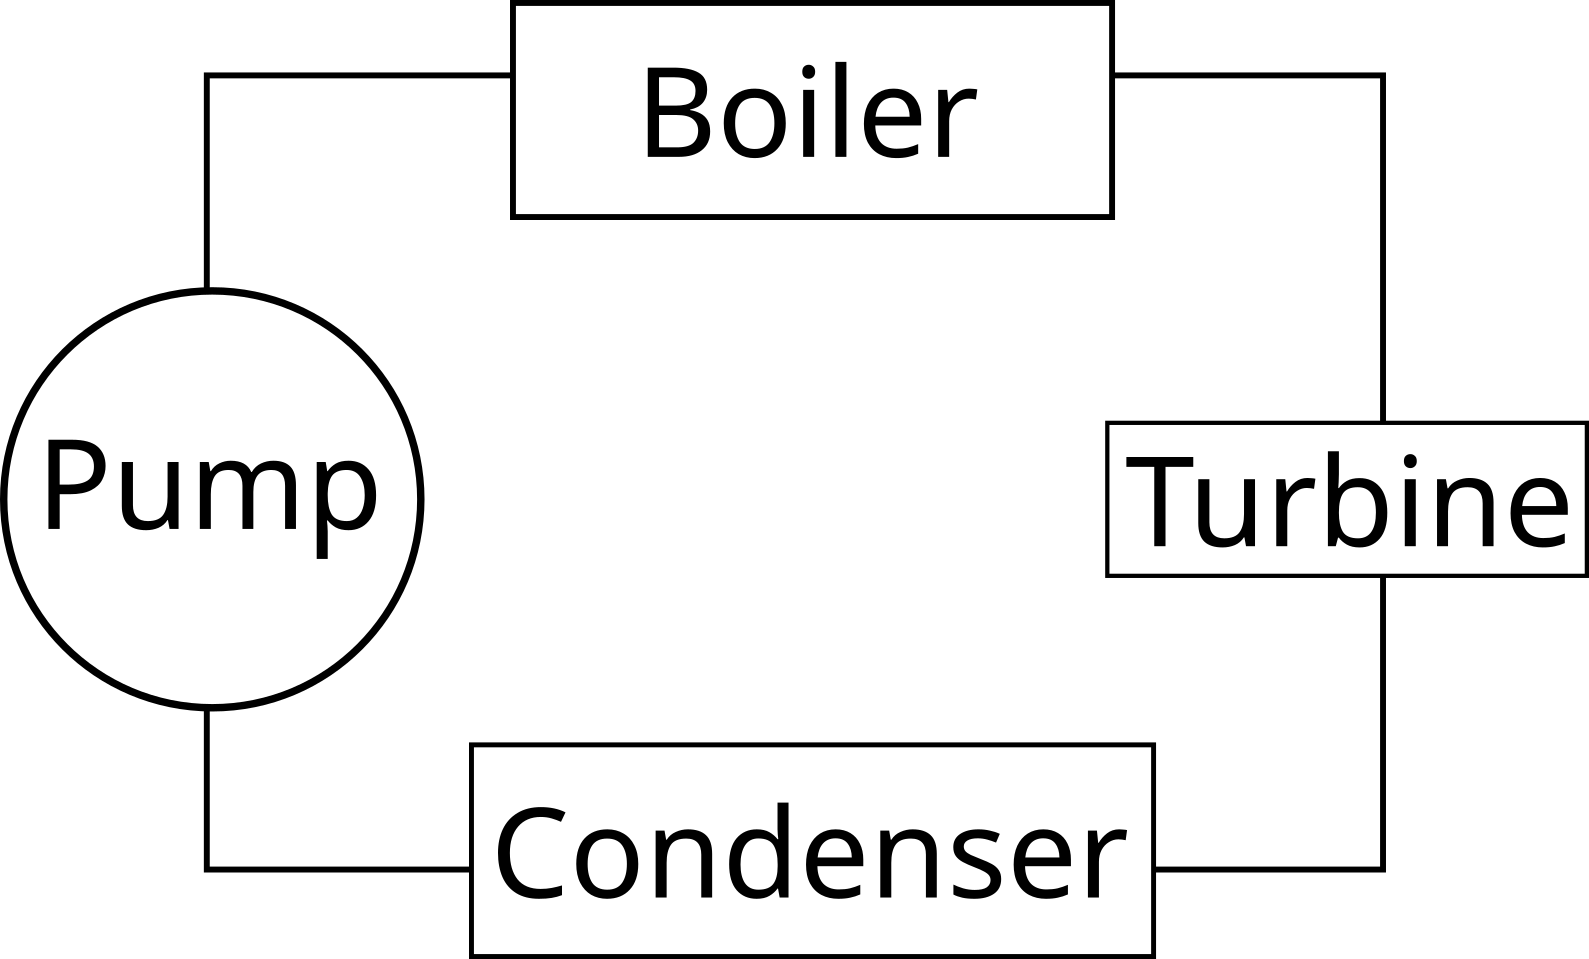
\includegraphics[scale=0.50]{./Heat_Engine_Schematic.png}
  % \input{./Drawings/MMAE_320-Thermo/Heat_Engine_Schematic.pdf_tex}
  \caption{Heat Engine}
  \label{fig:Heat_Engine}
\end{figure}

The boundary of the system is such that the entire system is contained.
This means that each element of the system is a different part of the thermodynamic energy balance.
\begin{itemize}[noitemsep]
\item The boiler takes the \nameref{def:Heat} in.
  Because this is typically the hot side of the \nameref{def:System}, we call this $\FlowRate{\Heat}_{H}$.
\item The turbine is for the \nameref{def:Work} out.
\item The condenser is for the \nameref{def:Heat} out.
  Because this is typically the cold side of the \nameref{def:System}, we call this $\FlowRate{\Heat}_{L}$.
\item The pump is for the \nameref{def:Work} in.
\end{itemize}

Thus, we can define the efficiency as shown in \Cref{eq:Energy_Efficiency-Heat_Engine}.
\begin{equation}\label{eq:Energy_Efficiency-Heat_Engine}
  \begin{aligned}
    \Efficiency &= \frac{\FlowRate{\Work}_{\text{Net Out}}}{\FlowRate{\Heat}_{H}} \\
    &= 1 - \frac{\FlowRate{\Heat}_{C}}{\FlowRate{\Heat}_{H}}
  \end{aligned}
\end{equation}

If we examine \Cref{eq:Energy_Efficiency-Heat_Engine}, we see that:
\begin{itemize}[noitemsep]
\item $\FlowRate{\Heat}_{H}$ sits on the boiler, which is at a higher temperature.
\item $\FlowRate{\Heat}_{C}$ sits on the condenser, which is at a lower temperature.
\end{itemize}
The greater the temperature difference between the system and its surroundings, the greater the efficiency of the \nameref{def:System}.

If there is no \nameref{def:Work} out, but work in is present, then \nameref{def:Energy} is being forced out of the lower temperature reservoir ($\FlowRate{\Heat}_{C}$) and put into the higher temperature reservoir.

\Cref{eq:Energy_Efficiency-Heat_Engine} is actually completely general.
It works for car engines, steam-based electricity generating power plants, refrigerators, heat pumps, etc.

\subsubsection{The Second Law and Heat Engines}\label{subsubsec:2nd_Law_Heat_Engines}
The \nameref{def:2nd_Law_Thermo} states that $\FlowRate{\Heat}_{C} = 0$ is impossible, for \nameref{def:Cycle}s.
If we think in terms of \nameref{rmk:Thermal_Reservoir}s, the second law states we cannot turn all the \nameref{def:Heat} provided by one reservoir into usable work.

However, $\FlowRate{\Heat}_{C} = 0$ \textbf{if the \nameref{def:Process} is NOT \nameref{rmk:Cyclic}}.

\begin{definition}[Coefficient of Performance]\label{def:Coefficient_of_Performance}
  The \emph{coefficient of performance} is a scalar value, like efficiency.
  It shows the relationship between a certain amount of \nameref{def:Energy} out given a certain amount of energy in.
  Or vice versa, it shows the potential output of the system given a certain input.

  \begin{equation}\label{eq:Coefficient_of_Performance}
    \CoP = \frac{\text{Desired Output}}{\text{Required Input}}
  \end{equation}
\end{definition}

Now, applying \nameref{def:Coefficient_of_Performance} to a heat engine, we get \Cref{eq:Coefficient_of_Performance-Heat_Engine}.

\begin{equation}\label{eq:Coefficient_of_Performance-Heat_Engine}
  \begin{aligned}
    \CoP &= \frac{\FlowRate{\Heat}_{C}}{\FlowRate{\Work_{Out}}} \\
    &= \frac{\FlowRate{\Heat}_{C}}{\FlowRate{\Heat}_{H} - \FlowRate{\Heat}_{C}} \\
    &= \frac{1}{\frac{\FlowRate{\Heat}_{C}}{\FlowRate{\Heat}_{H}} - 1}
  \end{aligned}
\end{equation}

\subsection{Heat Pumps}\label{subsec:Heat_Pumps}
\begin{definition}[Heat Pump]\label{def:Heat_Pump}
  A \emph{heat pump} is just another term for a refrigerator.
\end{definition}

\begin{example}[Textbook Problem 7.41]{Heat Pumps}
  A commercial \nameref{def:Heat_Pump} removes $\FlowRate{\Heat}_{C} = \SI{10000}{\btu\per\hour}$ from the source and rejects $\FlowRate{\Heat}_{H} = \SI{15090}{\btu\per\hour}$ to the sink, and has a $\FlowRate{\Work}_{In} = \SI{2}{\hp}$ of power.
  What is the \nameref{def:Coefficient_of_Performance}?
  \tcblower{}
  \textbf{Concepts:} \\
  A \nameref{def:Heat_Pump} is quite similar to a \nameref{def:Refrigerator}. \\
  The energy flow for the problem looks identical to a refrigerator's. \\
  A refrigerator has a \nameref{def:Coefficient_of_Performance} as seen in \Cref{eq:Coefficient_of_Performance-Refrigerator}.

  \textbf{Solve:} \\
  First, change the \nameref{def:Work} into a more useful set of units.
  \begin{equation*}
    \SI{2}{\hp} \left( \frac{\SI{2544}{\btu\per\hour}}{\SI{1}{\hp}} \right) = \SI{5088}{\btu\per\hour}
  \end{equation*}

  Now, we can solve \Cref{eq:Coefficient_of_Performance-Refrigerator}.
  \begin{align*}
    \CoP &= \frac{\FlowRate{\Heat}_{H}}{\FlowRate{\Work_{In}}} \\
         &= \frac{\SI{15090}{\btu\per\hour}}{\SI{5088}{\btu\per\hour}} \\
         &= 2.97
  \end{align*}
\end{example}

\begin{example}[Textbook Problem 7.48]{Air Conditioner}
  When a man returns to his well-sealed house on a summer day, he finds the house to be at $\Temp_{1} = \SI{32}{\degreeCelsius}$.
  He turns on the air conditioner which cools the entire house to $\Temp_{2} = \SI{20}{\degreeCelsius}$ in $\Time = \SI{15}{\minute}$.
  If the \nameref{def:Coefficient_of_Performance} of the air conditioning unit is $\CoP = 2.5$, determine the power drawn by the air conditioner?
  Assume the entire mass of the house is $\Mass = \SI{800}{\kilo\gram}$ of air for which $\SpecificHeatVolume = \SI{0.72}{\kilo\joule\per\kilo\gram\degreeCelsius}$ and $\SpecificHeatPressure = \SI{1.0}{\kilo\joule\per\kilo\gram\degreeCelsius}$.
  \tcblower{}
  \textbf{Concepts:} \\
  An air conditioner behaves the same as a \nameref{def:Refrigerator}. \\
  Continuing with this analogy, the air inside the house behaves as the interior of the refrigerator and is to be cooled.
  The air outside the house is analogous to the air outside of the refrigerator (the condenser is outside the house). \\
  Need to find $\FlowRate{\Heat}_{C}$.

  \textbf{Explore:} \\
  We can find the \nameref{def:Work} in by negating the change in \nameref{def:Heat} of the air inside the house.
  We can do this because the house is well-sealed and that is the only thing that can change the \nameref{def:Internal_Energy} of the house. \\
  \begin{equation*}
    -\FlowRate{\Work}_{In} = \frac{\FlowRate{\Heat}_{C}}{\CoP}
  \end{equation*}

  Because the house is well-sealed, if the air is cooled, the pressure will change.
  If the house were leaky, then air will flow somewhat freely across the system boundary.
  In this case, we will use $\SpecificHeatPressure$.

  More thoroughly, we will use both $\SpecificHeatVolume$ and $\SpecificHeatPressure$ to bracket our solution.
  \begin{equation*}
    \Change{\Heat} = \SpecificHeat \Mass \Change{\Temp}
  \end{equation*}

  We can use this to find the \nameref{def:Heat} removed from the house $\Heat_{C}$ and then determine its flowrate by dividing by the time taken, $\FlowRate{\Heat}_{C}$.

  \textbf{Plan:} \\
  Solve for the change in energy of the house using the equation for changes in heat given the fluid in question is an ideal gas.

  \textbf{Solve:} \\
  Starting with $\SpecificHeatVolume$ for a leaky house.
  \begin{align*}
    \Heat_{C, \Volume} &= \SpecificHeatVolume \Mass \Change{\Temp} \\
    &= \SI{6912}{\kilo\joule}
  \end{align*}

  Now, using $\SpecificHeatPressure$ for a well-sealed house.
  \begin{align*}
    \Heat_{C, \Pressure} &= \SpecificHeatPressure \Mass \Change{\Temp} \\
    &= \SI{9600}{\kilo\joule}
  \end{align*}

  Now, finding the flowrates.
  \begin{align*}
    \FlowRate{\Heat}_{C, \Volume} &= \SI{7.68}{\kilo\joule\per\second} & \Heat_{C, \Pressure} &= \SI{10.6}{\kilo\joule\per\second} \\
    \FlowRate{\Heat}_{C, \Volume} &= \SI{7.68}{\kilo\watt} & \Heat_{C, \Pressure} &= \SI{10.6}{\kilo\watt} \\
  \end{align*}

  Now, solving for the net \nameref{def:Work} in:
  \begin{align*}
    \FlowRate{\Work}_{In, \Volume} &= \SI{3.077}{\kilo\watt} & \FlowRate{\Work}_{In, \Pressure} &= \SI{4.264}{\kilo\watt}
  \end{align*}

  \textbf{Validate:} \\
  The sealed room doesn't take as much energy to cool, because we don't have to constantly cool newly warmed air from the outside, which makes sense.

  We can find $\FlowRate{\Heat}_{C}$ using \nameref{def:Enthalpy}, from Table A.21.
  \begin{align*}
    \FlowRate{\Heat} &= \Mass \Change{\SpecificEnthalpy} \\
                     &= \SI{9000}{\kilo\watt}
  \end{align*}

  Using the \nameref{def:Enthalpy} we can see that the best designed system is one that is between both the $\SpecificHeatVolume$ and $\SpecificHeatPressure$.
\end{example}

\subsection{Refrigerators}\label{subsec:Refrigerators}
In the case of a refrigerator (which is just a \nameref{fig:Heat_Engine} run in reverse), we get \Cref{eq:Coefficient_of_Performance-Refrigerator}.

\begin{definition}[Refrigerator]\label{def:Refrigerator}
  A \emph{refrigerator} takes \nameref{def:Work} in to remove \nameref{def:Heat} from its interior and moves it to the exterior.
\end{definition}

\begin{equation}\label{eq:Coefficient_of_Performance-Refrigerator}
  \begin{aligned}
    \CoP &= \frac{\FlowRate{\Heat}_{H}}{\FlowRate{\Work_{In}}} \\
    &= \frac{1}{1 - \frac{\FlowRate{\Heat}_{C}}{\FlowRate{\Heat}_{H}}}
  \end{aligned}
\end{equation}

\begin{example}[Textbook Problem 7.40]{Refrigerators}
  A household \nameref{def:Refrigerator} with a \nameref{def:Coefficient_of_Performance} of $\CoP = 1.2$ removes heat from the refrigerated space at a rate of $\FlowRate{\Heat}_{Out} = \SI{60}{\kilo\joule\per\minute}$.
  Determine the electric power consumed by the refrigerator ($\FlowRate{\Work}_{In}$) and the rate of \nameref{def:Heat_Transfer} to the kitchen air ($\FlowRate{\Heat}_{H}$)?
  \tcblower{}
  \textbf{Concepts:} \\
  A refrigerator has a \nameref{def:Coefficient_of_Performance} as seen in \Cref{eq:Coefficient_of_Performance-Refrigerator}. \\
  We are told $\FlowRate{\Heat}_{C} = \SI{60}{\kilo\joule\per\minute}$, which is $\FlowRate{\Heat}_{C} = \SI{1}{\kilo\joule\per\second}$. \\
  The $\FlowRate{\Heat}_{C}$ is the inside of the fridge and its air because of the evaporator.
  $\FlowRate{\Heat}_{H}$ is the warm air inside the kitchen and the air released by the condenser.

  \textbf{Explore:} \\
  From our simplified depiction of a refrigerator, we can figure out an energy balance for this problem, $\FlowRate{\Heat}_{H} = \FlowRate{\Heat}_{L} + \FlowRate{\Work}$.

  \textbf{Plan:} \\
  Solve \Cref{eq:Coefficient_of_Performance-Refrigerator} to find $\FlowRate{\Heat}_{H}$. \\
  Solve the energy balance to find $\FlowRate{\Work}_{In}$.

  \textbf{Solve:} \\
  Using \Cref{eq:Coefficient_of_Performance-Refrigerator}, solve for $\FlowRate{\Work}_{In}$.
  \begin{align*}
    \FlowRate{\Work}_{In} &= \frac{\FlowRate{\Work}_{C}}{\CoP} \\
                          &= \frac{\SI{1}{\kilo\joule\per\second}}{1.2} \\
                          &= \SI{50}{\kilo\joule\per\minute} \\
                          &= \SI{0.83}{\kilo\watt}
  \end{align*}

  Now, we can solve the energy balance.
  \begin{align*}
    \FlowRate{\Heat}_{H} &= \FlowRate{\Heat}_{C} + \FlowRate{\Work}_{In} \\
                         &= \SI{60}{\kilo\joule\per\minute} + \SI{50}{\kilo\joule\per\minute} \\
                         &= \SI{110}{\kilo\joule\per\minute}
  \end{align*}

  \textbf{Validate:} \\
  We cal validate this by double-checking against the general equation for \nameref{def:Coefficient_of_Performance} for a refrigerator, \Cref{eq:Coefficient_of_Performance-Refrigerator}.
  \begin{align*}
    \CoP &= \frac{1}{\frac{\FlowRate{\Heat}_{C}}{\FlowRate{\Heat}_{H}} - 1} \\
         &= 1.2
  \end{align*}

  \textbf{Generalize:} \\
  For a refrigerator, the higher the \nameref{def:Coefficient_of_Performance}, the more \nameref{def:Heat} removed from the inside.
\end{example}

\subsection{Reversible and Irreversible Processes}\label{subsec:Reversible_Irreversible_Processes}
\begin{definition}[Reversible Process]\label{def:Reversible_Process}
  A \emph{reversible process} is a thermodynamic \nameref{def:Process} that can reversed without affecting the system surroundings.
  This means the system is always in equilibrium.
\end{definition}


%%% Local Variables:
%%% mode: latex
%%% TeX-master: "../../MMAE_320-Thermo-Reference_Sheet"
%%% End:


%%% Local Variables:
%%% mode: latex
%%% TeX-master: "../MMAE_320-Thermo-Reference_Sheet"
%%% End:
